%  !TEX root = ../main.tex

\section{Background}
\subsection{Automatic Speech Recognition}\label{background_ASR}
Automatic speech recognition (ASR) systems, e.g., voice assistants, receive and recognize speech commands; then perform execution according to certain rules. 
Hidden Markov models (HMM)~\cite{baum1966statistical} and dynamic time warping (DTW)~\cite{berndt1994using} are two traditional statistical techniques for performing speech recognition.
With the development of deep learning, the end-to-end neural ASR models have gone mainstream, such as RNN-T~\cite{graves2012sequence} and DeepSpeech2~\cite{amodei2016deep}. 

A typical end-to-end ASR system pipeline includes four main components: \circled{1} \textit{Spectrum generator}: converts raw audio into spectrum features, e.g., Filter Bank (Fbank), Mel-Frequency Cepstral Coefficients (MFCC), etc. \circled{2} \textit{Neural acoustic model}: takes spectrums as input and outputs a matrix of probabilities over linguistic units (e.g., phoneme, syllable, or word) over time. For instance, English ASR is widely modeled with 29 basic units (also known as tokens), including characters a\textasciitilde z, space, apostrophe, and blank symbol $\phi$. \circled{3} \textit{Decoder}: generates possible sentences from the probability matrix, also optionally coupled with an n-gram language model to impose word-level constraints. The Connectionist Temporal Classification (CTC) module is a typical decoder that sums over all possible alignments that may reduce to the same token sequence, whereby ``o$\phi$kk$\phi$a$\phi$y'' and ``o$\phi$k$\phi$aa$\phi$yy'' are regarded as the same ``okay''. \circled{4} \textit{Punctuation and capitalization model}: formats the generated text for easier human consumption.

\subsection{Audio Adversarial Examples}
Adversarial examples (AEs)~\cite{carlini2018audio,schonherr2018adversarial,yuan2018commandersong,chen2020metamorph} use specialised inputs created with the purpose of confusing a neural network, resulting in the misclassification of a given input. In the audio domain, by adding a crafted perturbation $\delta$ with some constraints $\epsilon$ throughout the original benign audio $x$, the ASR model will be fooled to transcribe a perturbed speech into the targeted text $y_t$, e.g., ``take the picture''. To craft an adversarial example, an adversary may leverage the optimization function:
% \vspace{-5pt}
\begin{equation}
\begin{aligned}
    & {minimize}~ \mathcal{L}(f(x+\delta), y_t) + \alpha\cdot\Vert{\delta}\Vert_{p}\\
    % & {s.t.}~ \delta \in [-\epsilon, \epsilon]^n, (\text{e.g.,}~\epsilon\textless 0.01)
    & {s.t.}~ \delta \in [-\epsilon, \epsilon]^n, (\epsilon\textless 0.01)
\end{aligned}
\label{equ:audible_ae_formula}
% \vspace{-10pt}
\end{equation}
where the ASR functions as $f(\cdot)$ that takes an input waveform and outputs the probability matrix. $\mathcal{L}(f(\cdot),y_t)$ is the CTC loss function denoting the distance between the model output of the adversarial example and the target. $\|\cdot\|_{p}$ means the $L_p$ norm. $\alpha$ is a penalty term to limit the $L_p$. $\epsilon$ denotes the upper bound of the perturbation. 
Recently, the concept of universal adversarial perturbation is proposed, making AEs valid regardless of the user commands.
To make the AEs more concealed, the creating approaches are extended to psychoacoustic hiding~\cite{schonherr2018adversarial,qin2019imperceptible} and shorter pulses~\cite{li2020advpulse}. However, existing efforts cannot fundamentally avoid being perceived by human ears.

\begin{figure}[t]
	\centering
	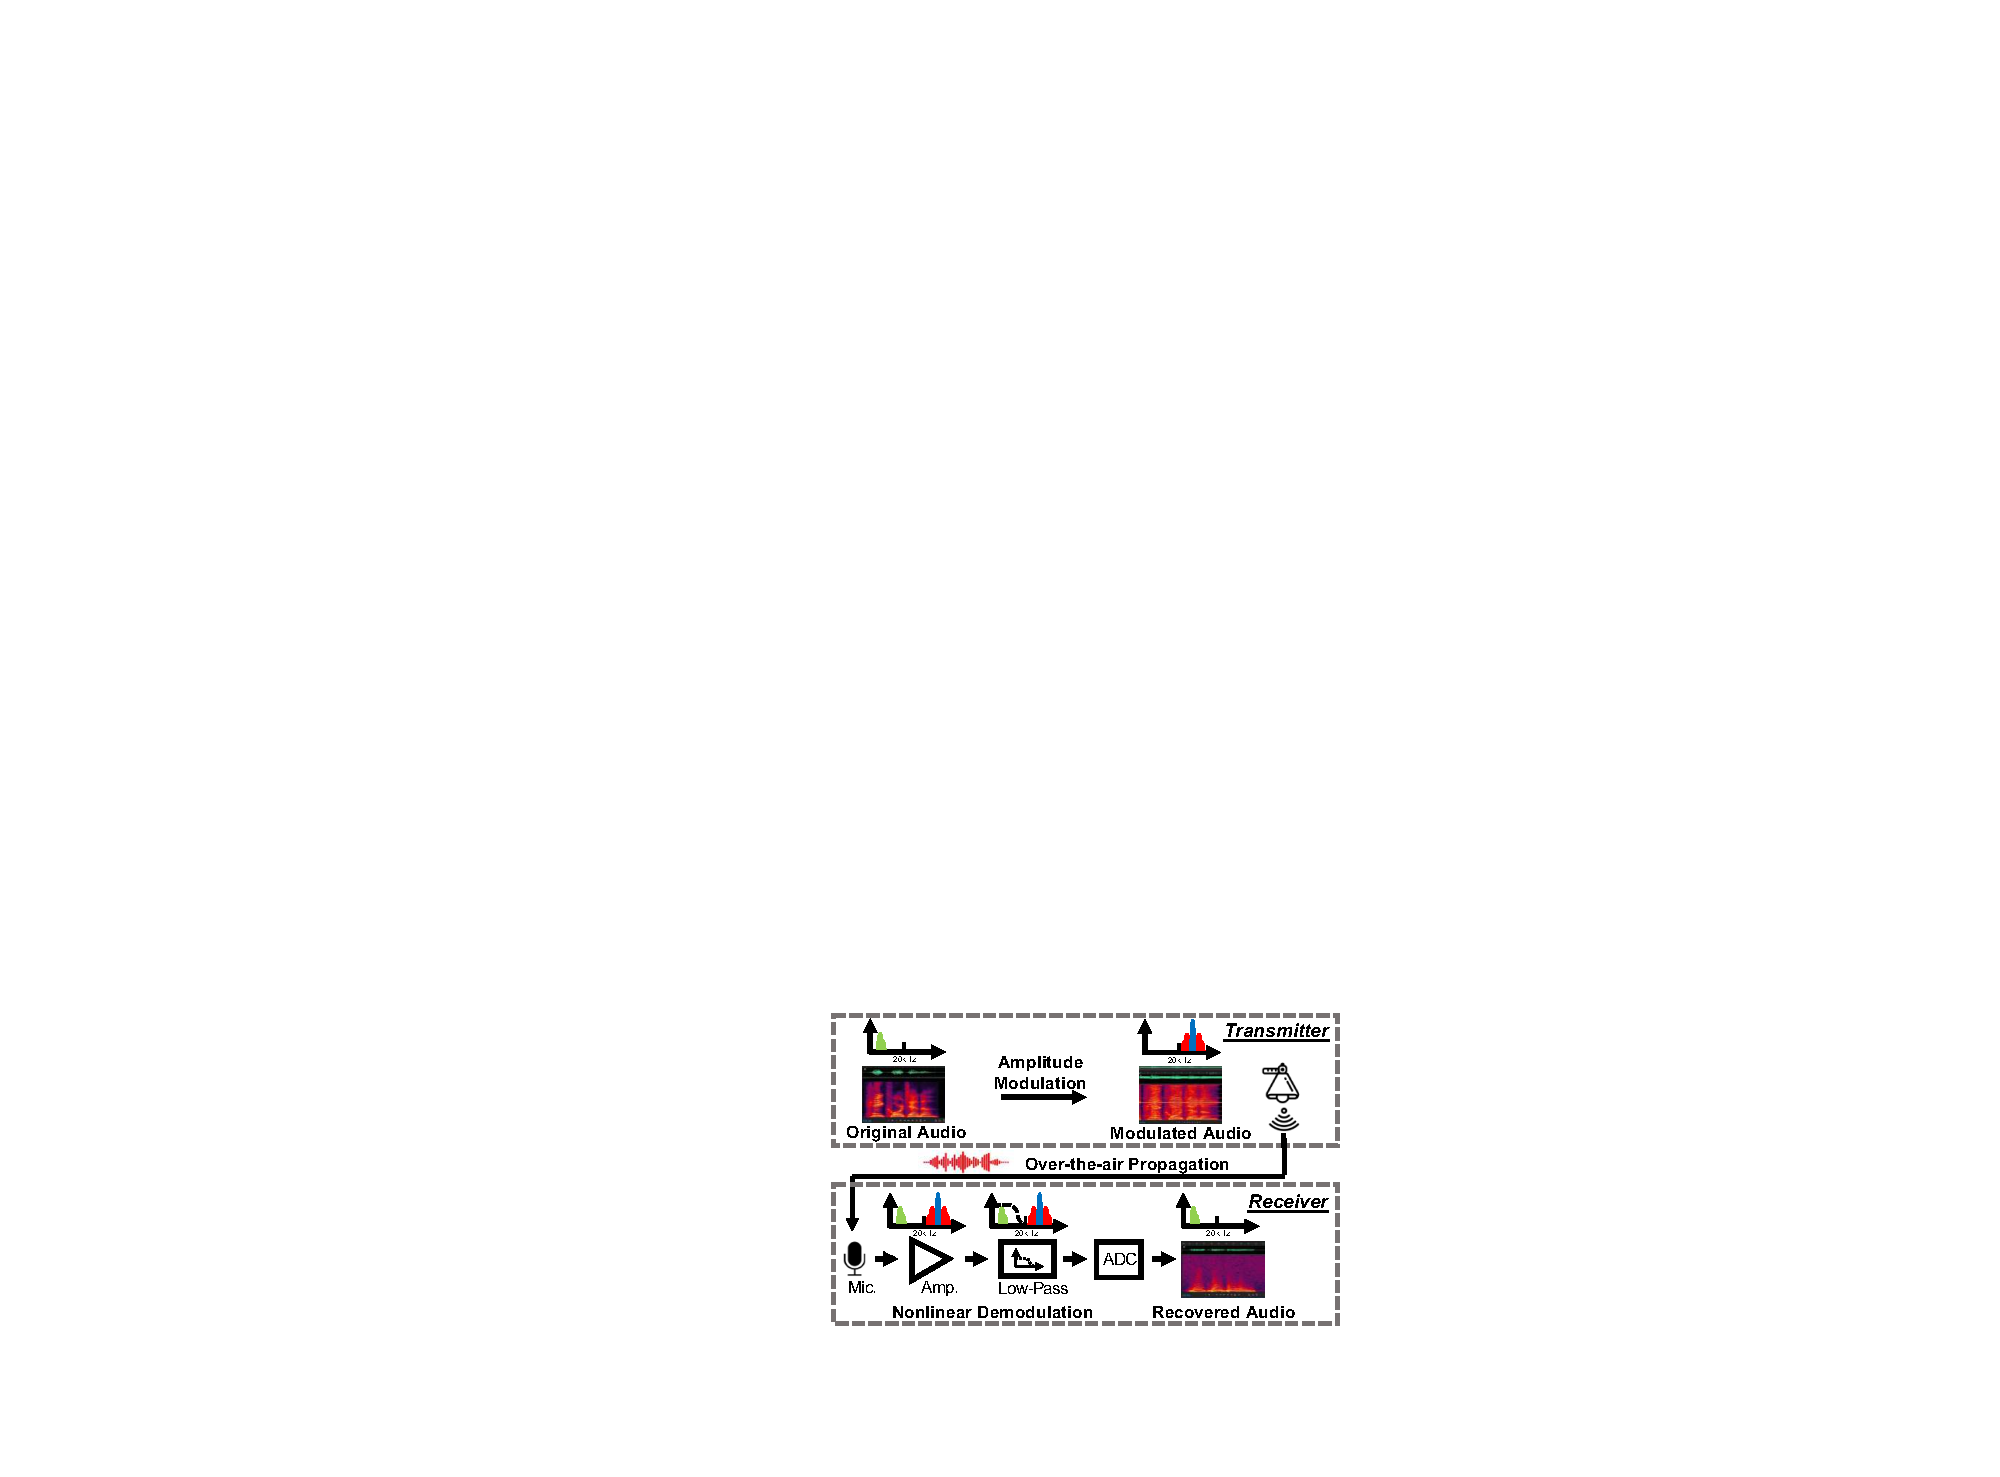
\includegraphics[width=0.4\textwidth]{background_inattack.pdf}
	\caption{\label{fig:dolphinattack_pipeline}Diagram of inaudible attacks (carrier: blue, baseband: green).}
	% \vspace{-10pt}
        \addvspace{-15pt}
\end{figure}



\subsection{Ultrasound-based Attacks}\label{background_vulnerability_VCS}
Inaudible attacks modulate the audio baseband on high-frequency carriers to the inaudible band of human ears ($>$20~kHz) and exploit microphones' nonlinear vulnerability, so that ASRs can receive the malicious audio while humans cannot perceive it.
Recently, inaudible attacks have been extended from ultrasonic carrier~\cite{zhang2017dolphinattack,roy2018inaudible} to various forms, such as solid conduction~\cite{yan2020surfingattack}, laser~\cite{sugawara2020light}, capacitor~\cite{zhang2021capspeaker}, power line~\cite{wang2022ghosttalk}, etc., forming a class of highly threatening and comprehensive covert attacks. % Such attacks have posed serious challenges to the security of ASRs, user information privacy, etc.
We take the representative ultrasound-based attack~\cite{zhang2017dolphinattack} to present the principle of inaudible attacks shown in Fig.~\ref{fig:dolphinattack_pipeline}.
First, the original audio is double-sideband (DSB) modulated on an ultrasound carrier via amplitude modulation (AM). Second, the DSB-AM audio is emitted from the ultrasonic transducer and propagates over the air. Third, after the microphone receives the signal, audio modulated on the high-frequency carrier will be recovered into the audible band \textit{before the low-pass filters and ADC} due to nonlinear effects of the microphone's diaphragm and amplifier. Thus, though the ultrasound carrier is finally filtered, the demodulated audio still survives and functions to ASR.
The nonlinear demodulation is formulated as follows: 
\begin{equation}\label{equ:nonlinearity}
    S_{out}(t) = \sum_{i=1}^{\infty}k_{i}s^{i}(t)=k_1 s(t) + k_2 s^2(t) + k_3 s^3(t) + ...
\end{equation}
where $s(t)$ and $S_{out}(t)$ indicate the input AM signal and amplifier's output, respectively. %The third and higher order terms are extremely weak and can be ignored, and 
The even order terms, i.e., $k_2$, $k_4$ are the key in recovering the original audio~\cite{roy2017backdoor}.
Notably, such an ultrasound channel is lossy as the recovered audio samples differ from original ones. Our investigation demonstrates that the channel is also challenging to model~\ref{sec:ultrasound_observation}.